
\chapter{Autograders}
\label{chapter:autograders}

The incorporation of autograders within Verilog/SystemVerilog education is arguably the most valuable aspect of RTL education. These tools, particularly exemplified by platforms like Gradescope, can introduce a dynamic and interactive dimension to the learning process, revolutionizing the way students engage with Verilog concepts. Leveraging custom docker containers and custom Bash scripts, Gradescope's autograders easily facilitate Verilog testbench simulations, strict linting, synthesis, gate-level simulation, and more, yielding insights and feedback on various aspects of student submissions. However, managing software licenses on autograder servers can be a hassle, so all these functionalities are often best deployed with open-source tools. In the context of UCSB's ECE 152A, 154A, and 154B courses, students responded extremely positively to autograders, visibly enhancing their mastery over synthesizable Verilog.

\section{Autograders offer instant, high-quality feedback.}

Students are empowered to submit their code multiple times, enabling them to refine their solutions and learn from their mistakes in real time. This back-and-forth approach ensures that students can practice a Verilog concept and receive as much help as they need until they pass all the instructor-defined tests. In the autograders that I set up, it's worth noting that a significant majority of students eventually achieve a 100\% score by the assignment deadline. Therefore, autograders fall under the educational approach known as \enquote{Ungrading,} where the emphasis shifts strongly toward providing valuable feedback over assigning traditional grades. This phenomenon essentially transforms the grading system into a confidence-building mechanism rather than a competitive ranking system. Ungrading has been shown to help students by reducing stress, inspiring creativity, and encouraging healthy risk taking. \cite{kohn:book, blum:article} However, arguably Ungrading's largest downside is that the instructor may not have time to provide personalized feedback to all students. Fortunately, an intrinsic attribute of software, (such as HDL implementations), is that code quality and correctness can be run with automatic, subjective computer algorithms. Therefore, by implementing autograders, Verilog educators can easily tap into this pedagogical insight, offering students a more effective way to grasp digital design principles.

\section{Autograders can run remotely without complex local-setup.}
\label{section:complex_tool_setups}

When instructing students on crafting Verilog code that maintains accurate synthesizability across various platforms, it is essential to follow the industry standard of verifying a design with a wide selection of tools. Autograders streamline this process, making it accessible and efficient for students to perform comprehensive testing without the need for local installation. For example, the autograders that I created for ECE 152A, 154A, and 154B would consistently use anywhere from 6 to 10 different tools, sometimes requiring complex installation and setup procedures. Expecting students to complete these setup procedures is often tedious and counterproductive. Therefore, simply giving students access to a fully prepared autograder can remove the setup barrier completely.

As mentioned, an autograder test suite that closely mirrors industry quality should follow all the verification steps demonstrated in \autoref{fig:asic_flow}. First, it is important to run behavioral simulations with multiple tools such as Icarus, which supports propagation of unknown (\mintinline{SystemVerilog}{x}) values, and simulation with Verilator, which has stronger restrictions on bad syntax. Only by passing simulations with both tools should the autograder grant full points. Furthermore, code linters such as Verilator and Verible can ensure adherence to essential coding standards and practices, checking for issues like latches in \mintinline{SystemVerilog}{always_comb} blocks, correct use of blocking and non-blocking assignments, net-width discrepancies, and more. Considering that the frontends of tools do not always offer helpful warnings, this detailed syntax checking from Verilator and Verible is invaluable for students when fixing otherwise cryptic issues. Then, to deploy SystemVerilog synthesis with open-source tools, Yosys and Nextpnr must be paired with a frontend such as Surelog or zachjs/sv2v. The Yosys synthesis and Nextpnr layout process can verify if students are using too many logic cells, if their design is too slow, or if their design infers prohibited logic cells. As a final post-synthesis step, Icarus can be run one final time on the Yosys output to initiate a gate-level simulation (GLS) with unknown value propagation, and Yosys EQY can be run to perform logical equivalence checking (LEC). All of these features\footnote{Inclusion of LEC with EQY into an autograder remains outstanding due to time constraints during the project's development.} have been successfully implemented in autograders for ECE 152A, 154A, and 154B.

\section{\enquote{For-fun} leaderboards can excite and inspire students.}
\label{section:leaderboard}


\begin{figure}[t]
    \centering
    \frame{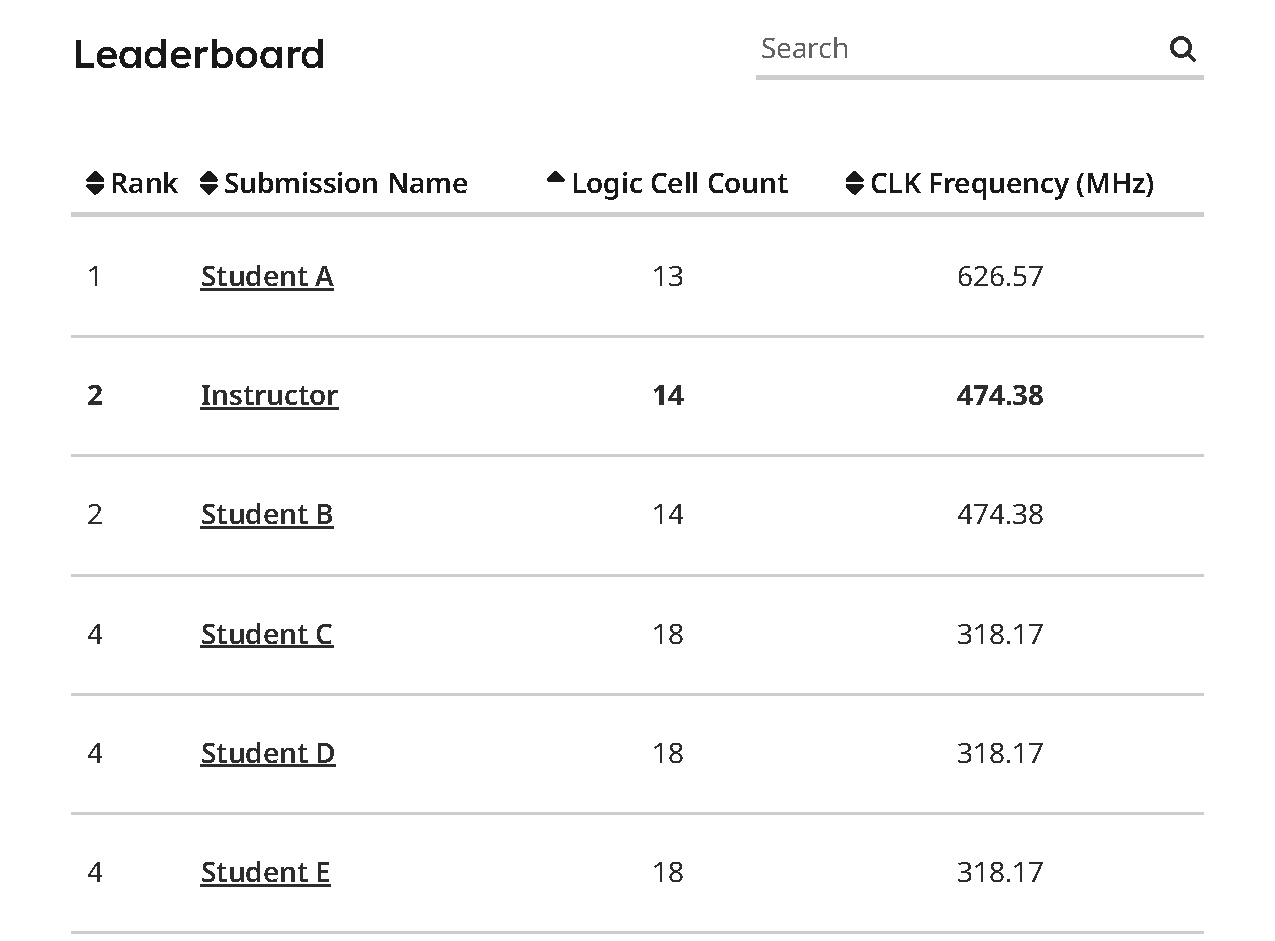
\includegraphics[width=0.8\linewidth]{media/graphics/leaderboard.pdf}}
    \caption[
        Gradescope Leaderboard
    ]{
        Example of a Gradescope leaderboard for a counter lab (same lab as in \autoref{fig:unreadable_opt}).
        Student designs were ranked on cell usage and maximum frequency as calculated by Yosys and Nextpnr-ice40.
        (Student names have been obfuscated for privacy reasons).
    }
    \label{fig:leaderboard}
\end{figure}


\begin{figure}[t]
    \centering
    \inputminted[frame=single]{systemverilog}{code/unreadable_opt.svh}
    \caption{Student drastically reduced readability and transferability in order to save 1 logic cell over the teacher solution.}
    \label{fig:unreadable_opt}
\end{figure}


Aside from a grade assigned by the autograder, another form of feedback can be provided through a class leaderboard. Students can see how their submission compares to the rest of the class on statistics such as logic cell usage, max clock frequency, or branch predictor hit percentage (see \autoref{fig:leaderboard}). Since the leaderboards in ECE 152A and 154B didn't count towards any points, students really enjoyed seeing how each of their designs compared to their peers' designs, then would try to beat their friends for bragging rights. Because of this, I added leaderboards to every assignment that I could. However, it is important to clarify to students that code readability should be prioritized over moving up in the leaderboard by saving 1-2 logic cells. However, because autograders running purely open-source tools must only rely on Yosys and ABC for synthesis, students may be incorrectly rewarded for submissions that are not well-optimized for other more prevalent synthesis tools such as Design Compiler or Vivado (similar to \autoref{section:optimizations_in_netlist_graph_viewers}). This was a rare edge case that only visibly affected 1 submission (\autoref{fig:unreadable_opt}) across the 600+ leaderboard submissions I saw, but it is still important to monitor in students. Overall, creating assignment leaderboards was a great way to increase student enthusiasm without bringing additional stress or responsibilities.

\section{Autograders can foster community and collaboration.}

In ECE 152A, students discussed their challenges, insights, and strategies with peers, creating a collective learning environment. Since each student had a clear goal of \enquote{passing all the tests}, we saw students combine strategies and knowledge with confidence. Plus, ungraded leaderboards offered a fun but optional way for students to collaborate in friendly competitions. Communal engagement not only strengthens individual understanding, but also enriches the overall learning ecosystem. By integrating autograders, students experience a much more positive learning environment while still being provided critical skills and insights for their future engineering endeavors.
